\documentclass{article}
\usepackage[T1]{fontenc} % codificação da fonte em 8-bits
\usepackage[utf8]{inputenc} % acentuação direta
\usepackage[brazil]{babel} % em portugues brasileiro
\usepackage[normalem]{ulem}
\useunder{\uline}{\ul}{}
\usepackage{graphicx}
\usepackage[utf8]{inputenc}
\usepackage{fullpage}
\usepackage{listings}
\usepackage{xcolor}
\usepackage{amsmath}
\usepackage{amssymb}
\usepackage{url}
\usepackage{hyperref}
\usepackage[linesnumbered,ruled,vlined]{algorithm2e}
% \usepackage{enumitem}
\usepackage[shortlabels]{enumitem}
\usepackage{listings}
\lstset { %
    language=C++,
    backgroundcolor=\color{black!5}, % set backgroundcolor
    basicstyle=\footnotesize,% basic font setting
}

\definecolor{mygreen}{rgb}{0,0.6,0}

% set the default code style
\lstset{
    language=C++,
    frame=tb, % draw a frame at the top and bottom of the code block
    tabsize=4, % tab space width
    showstringspaces=false, % don't mark spaces in strings
    numbers=none, % display line numbers on the left
    commentstyle=\color{mygreen}, % comment color
    keywordstyle=\color{blue}, % keyword color
    stringstyle=\color{red}, % string color
    backgroundcolor=\color{black!5}, % set backgroundcolor
    basicstyle=\footnotesize,% basic font setting
    literate = {-}{-}1, % <------ trick for '-' in shell commands
}

\parindent0in
\pagestyle{plain}
\thispagestyle{plain}

\newcommand{\assignment}{Lista 6}
\newcommand{\duedate}{4 de abril}


\title{Lista 5}
\date{}

\begin{document}

Fundação Getulio Vargas\hfill\\
Estruturas de Dados\hfill\textbf{\assignment}\\
Prof.\ Jorge Poco\hfill\textbf{Entrega:} \duedate\\
\smallskip\hrule\bigskip

{\let\newpage\relax\maketitle}
\maketitle

\section{Questões Teóricas}

\paragraph{Problema 1.} (25 pontos)

Considerando o posicionamento dos pontos da Fig.~\ref{fig:prob1}:

\begin{figure}[h]
    \centering
    \includegraphics[width = 0.5\linewidth]{figs/fig1.png}
    \caption{Divisão do espaço em quadrantes de acordo com um conjunto de pontos.}
    \label{fig:prob1}
\end{figure}

\begin{itemize}
    \item a) Desenhe a \texttt{quadtree} que representa essa divisão do espaço em quadrantes.
    \item b) Remova o ponto $B$ dessa árvore e apresente os passos.
\end{itemize}

\paragraph{Resposta 1.}

\begin{figure}[h]
    \centering
    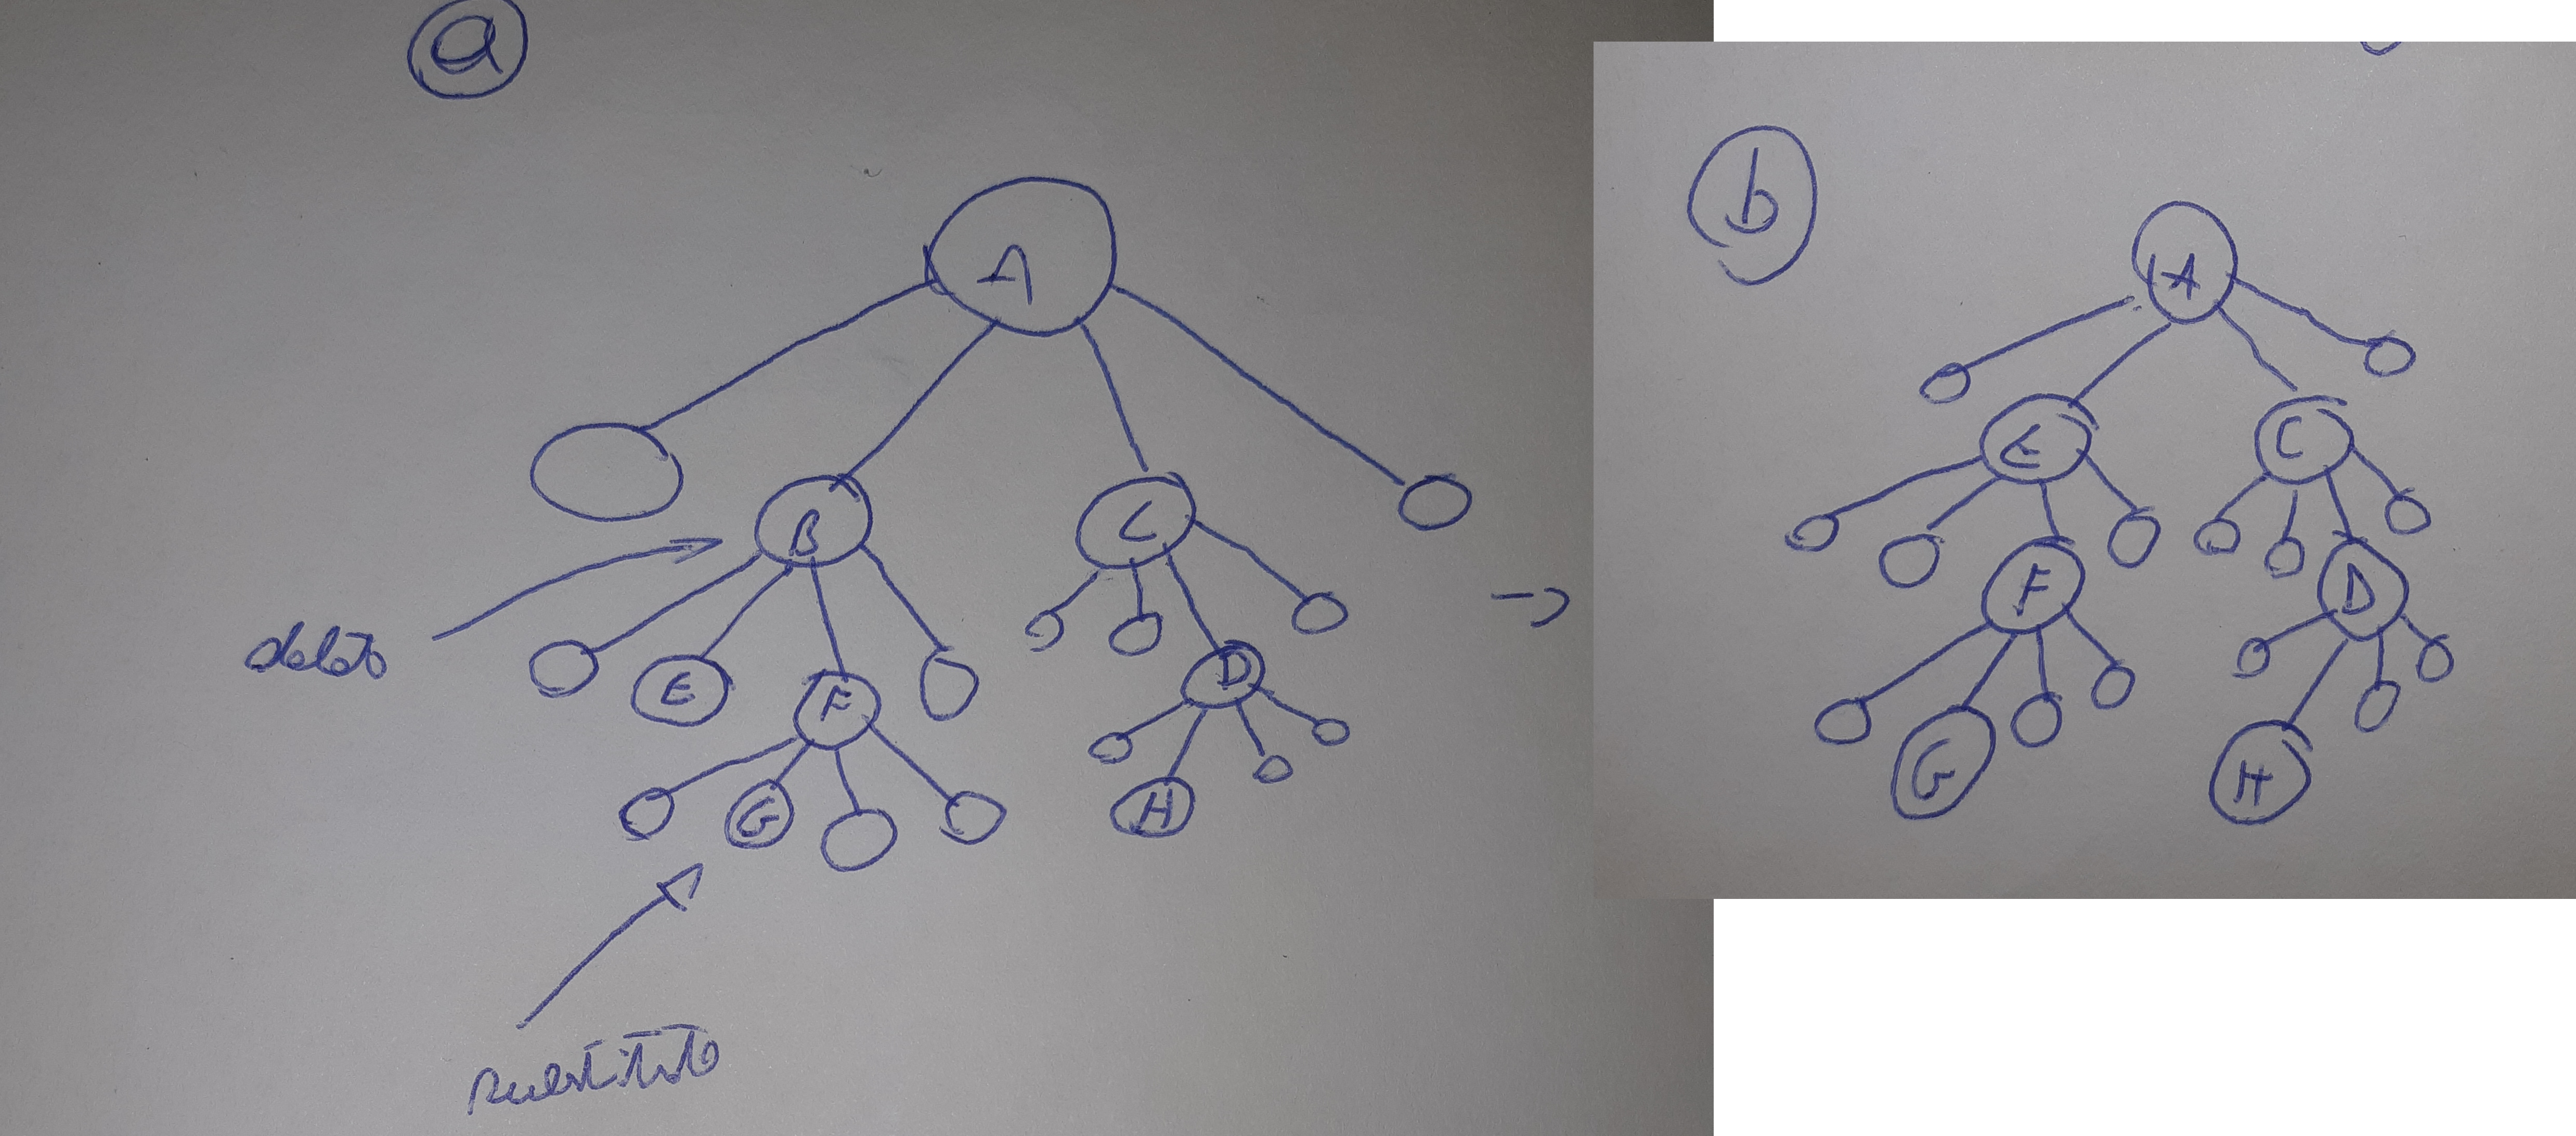
\includegraphics[width = 1.0\linewidth]{figs/fig5.png}
    \caption{\texttt{quadtree}}
    \label{fig:prob2}
\end{figure}


\paragraph{Problema 2.} (25 pontos)

Remova o elemento $(35, 60)$ da seguinte \textit{kd-tree} (Fig.~\ref{fig:prob2}) e apresente os passos.

\begin{figure}[h]
    \centering
    \includegraphics[width = 0.4\linewidth]{figs/fig2.png}
    \caption{\texttt{kd-tree}}
    \label{fig:prob2}
\end{figure}

\paragraph{Resposta 2.}

\begin{figure}[h]
    \centering
    \includegraphics[width = 1.0\linewidth]{figs/fig4.png}
    \caption{\texttt{delete (35,60)}}
    \label{fig:prob2}
\end{figure}

\paragraph{Problema 3.} (25 pontos) 

Neste problema veremos como usar \textit{kd-trees} para responder a uma consulta geométrica comum, chamado "tiro de raio" (\textit{ray shoot}). Você recebe um conjunto de segmentos verticais no espaço 2D, cada um
começa no eixo $x$ e vai até um ponto no quadrante positivo. Seja $P = \{p_1, . . . , p_n\}$ as extremidades superiores desses segmentos (ver Fig.~\ref{fig:prob3}). Todas as coordenadas são positivas.

\begin{figure}[h]
    \centering
    \includegraphics[width = 0.8\linewidth]{figs/fig3.jpeg}
    \caption{Pontos $P$ e o resultado de \texttt{rayShoot}.}
    \label{fig:prob3}
\end{figure}

Dado um ponto $q$, disparamos um raio horizontal que emana de $q$ para a direita. Este raio viaja
até atingir um desses segmentos (ou talvez erre todos). Por exemplo, na figura
acima, o raio disparado de $q$ atinge o segmento com ponto final superior $p_8$. O raio disparado de $q'$ não atinge nada.

Neste problema, mostraremos como responder a essas consultas usando uma \textit{kd-tree}. A consulta recebe o ponto $q = (q_x, q_y)$ e retorna o ponto final superior
$p_i \in P$ do segmento que o raio atinge primeiro, ou \texttt{null} se o raio erra todos os segmentos. 

Suponha que você receba uma \textit{kd-tree} de altura $O(\log n)$ armazenando os pontos de $P$ (não armazena os segmentos, apenas os pontos). Apresente pseudo-código para um algoritmo eficiente \texttt{rayShoot(q)},
que retorna uma resposta para a consulta de disparo de raio horizontal (veja a figura acima, à direita).

Você pode assumir que na estrutura cada nó armazena um ponto \texttt{p.point} (com duas coordenadas),
uma dimensão de corte \texttt{p.cutDim}, e ponteiros filhos esquerdo e direito \texttt{p.left} e \texttt{p.right}, respectivamente.

Você pode fazer uso de quaisquer operações primitivas em pontos e retângulos (mas por favor
explicá-los). Você pode assumir que não há valores de coordenadas duplicados entre os pontos de $P$ ou o ponto de consulta.

\paragraph{Resposta 3.}

\begin{lstlisting}
Point rayShoot(Point q, KDNode p, Rectangle cell, Point best) {
if (p == null) // caiu da arvore?
return best
else if (cell.high.x < q.x || cell.high.y < q.y) // sem sobreposicao
return best
else {
if (p.point.x >= q.x && p.point.y >= q.y && p.point.x < best.x)
best = p.point // p.point e o novo melhor
// obter filhos
Rectangle leftCell = cell.leftPart(p.cutDim, p.point)
Rectangle rightCell = cell.rightPart(p.cutDim, p.point)
if (cell.lo.y >= q.y && p.cutDim == 0) {
if (p.point.x > q.x) // nao precisa procurar a direita
best = rayShoot(q, p.left, leftCell, best)
else // no need to search left
best = rayShoot(q, p.right, rightCell, best)
} else {
best = rayShoot(q, p.left, leftCell, best)
best = rayShoot(q, p.right, rightCell, best)
}
return best;
}
}
\end{lstlisting}

O tempo de execução do algoritmo é O($\sqrt{n}$) sob a suposição de que a árvore esteja balanceada. Isso decorre da observação de que, para nós recorrermos em um nó, sua célula deve ser perfurada pelo linha vertical que passa pelo q ou pela linha horizontal que passa pelo q, e, como mostrado na aula, no tempo máximo de O($\sqrt{n}$) nós temos essa propriedade.

\paragraph{Problema 4.} (25 pontos)

chainingVocê tem uma tabela de \textit{hash} de tamanho $m$ na qual você insere $n$ chaves usando
"encadeamento" (\textit{separate chaining}). As chaves são inteiros selecionados do conjunto $U = \{1, 2, \dots , nm\}$.

\begin{enumerate}[label=\alph*)]
    \item Prove que, não importa quão engenhosamente você projete sua função \textit{hash},
deve existir um subconjunto $S$ de $U$ de tamanho pelo menos $n$ tal que cada chave em $S$ "\textit{hashes}" (mapeie) para a mesma localização na tabela de \textit{hash}.
    \item O que o item anterior implica sobre o tempo de execução do pior caso necessário para inserir $n$ chaves extraídas de $U$ em sua tabela de \textit{hash}.
\end{enumerate}

\paragraph{Resposta 4.}

(a) Isto segue-se por uma aplicação direta do princípio de pigeonhole Se distribuirmos nm chaves pelas m entradas da tabela de hash, pelo menos uma das entradas deve conter pelo menos n chaves. Selecione qualquer uma dessas entradas da tabela e deixe S denotar o subconjunto de chaves que foram 'hash' para esta entrada. Este subconjunto satisfaz as propriedades desejadas.
\\
\\
(b) Se tivermos a má sorte do usuário inserir todos os elementos de S na tabela de hash, eles todos irão 'hash' para o mesmo local e serão adicionados à mesma linked list. Quando o iº elemento de S for adicionado, precisaremos de O(i) tempo para percorrer a linked list (o que é necessário para verificar se não há duplicatas). Assim, o tempo total de inserção é proporcional a $\sum\limits_{i = 1i}^{n}i = O(n2)$


\section{Detalhes avaliação}
Uma pergunta comum é "quanto detalhe é esperado nas respostas?", algumas orientações são:
%
\paragraph{Provar vs. Mostrar:}
Se lhe pedirmos para “provar” algo, estamos à procura de uma prova bem estruturada. Se você estiver aplicando a indução, tenha cuidado para distinguir seu(s) caso(s) básico(s) e indicar qual é a sua hipótese de indução. Se lhe pedirmos para “mostrar”, “explicar” ou “justificar”, estaremos geralmente apenas esperando uma explicação em português. Se você não tiver certeza, por favor, verifique.

\paragraph{Algoritmo vs. Pseudocódigo:} Quando pedimos um “algoritmo” estamos esperando uma descrição em alto nível de algum processo computacional, geralmente em uma combinação de português e notação matemática (por exemplo, “classifique as $n$ chaves e localize $x$ usando busca binária”). Para pseudocódigo, nós estão esperando uma descrição passo a passo mais detalhada que se pareça muito mais com C++ (por exemplo, “\texttt{Node q = p.left}”). Lembre-se de que você está escrevendo seu código para ser lido por um humano, e não por um compilador. Por favor, omita detalhes irrelevantes que são sintaxes de C++. Mesmo que não solicitemos explicitamente, sempre que você fornecer um algoritmo ou pseudocódigo, você deve sempre fornecer uma breve explicação em português. Isso ajuda o avaliador a entender quais são suas intenções, e se houver um pequeno erro em seu código, muitas vezes podemos usar seu explicação para entender quais eram suas reais intenções.

\end{document}
